%%%%%%%%%%%%%%%%%%%%%%%%%%%%%%%%%%%%%%%%%
% baposter Landscape Poster
% LaTeX Template
% Version 1.0 (11/06/13)
%
% baposter Class Created by:
% Brian Amberg (baposter@brian-amberg.de)
%
% This template has been downloaded from:
% http://www.LaTeXTemplates.com
%
% License:
% CC BY-NC-SA 3.0 (http://creativecommons.org/licenses/by-nc-sa/3.0/)
%
%%%%%%%%%%%%%%%%%%%%%%%%%%%%%%%%%%%%%%%%%

%This template was modified by Patrick Nichols

%----------------------------------------------------------------------------------------
%	PACKAGES AND OTHER DOCUMENT CONFIGURATIONS
%----------------------------------------------------------------------------------------

\documentclass[landscape,a0paper,fontscale=0.285]{baposter} % Adjust the font scale/size here

\usepackage{graphicx} % Required for including images
\graphicspath{{figures/}} % Directory in which figures are stored

\usepackage{amsmath} % For typesetting math
\usepackage{amssymb} % Adds new symbols to be used in math mode

\usepackage{booktabs} % Top and bottom rules for tables
\usepackage{enumitem} % Used to reduce itemize/enumerate spacing
\usepackage{palatino} % Use the Palatino font
\usepackage[font=small,labelfont=bf]{caption} % Required for specifying captions to tables and figures

\usepackage{multicol} % Required for multiple columns
\setlength{\columnsep}{1.5em} % Slightly increase the space between columns
\setlength{\columnseprule}{0mm} % No horizontal rule between columns

\usepackage{tikz} % Required for flow chart
\usetikzlibrary{shapes,arrows} % Tikz libraries required for the flow chart in the template

\usepackage{listings}

\newcommand{\compresslist}{ % Define a command to reduce spacing within itemize/enumerate environments, this is used right after \begin{itemize} or \begin{enumerate}
\setlength{\itemsep}{1pt}
\setlength{\parskip}{0pt}
\setlength{\parsep}{0pt}
}

\definecolor{lightblue}{rgb}{0.145,0.6666,1} % Defines the color used for content box headers

\begin{document}

\begin{poster}
{
headerborder=closed, % Adds a border around the header of content boxes
colspacing=1em, % Column spacing
bgColorOne=white, % Background color for the gradient on the left side of the poster
bgColorTwo=white, % Background color for the gradient on the right side of the poster
borderColor=lightblue, % Border color
headerColorOne=black, % Background color for the header in the content boxes (left side)
headerColorTwo=lightblue, % Background color for the header in the content boxes (right side)
headerFontColor=white, % Text color for the header text in the content boxes
boxColorOne=white, % Background color of the content boxes
textborder=roundedleft, % Format of the border around content boxes, can be: none, bars, coils, triangles, rectangle, rounded, roundedsmall, roundedright or faded
eyecatcher=true, % Set to false for ignoring the left logo in the title and move the title left
headerheight=0.1\textheight, % Height of the header
headershape=roundedright, % Specify the rounded corner in the content box headers, can be: rectangle, small-rounded, roundedright, roundedleft or rounded
headerfont=\Large\bf\textsc, % Large, bold and sans serif font in the headers of content boxes
%textfont={\setlength{\parindent}{1.5em}}, % Uncomment for paragraph indentation
linewidth=2pt % Width of the border lines around content boxes
}
%----------------------------------------------------------------------------------------
%	TITLE SECTION 
%----------------------------------------------------------------------------------------
%
{
\includegraphics[height=4em]{NEMOS-logo.png}} % First university/lab logo on the left
{\bf\textsc{EasyUnlock: A Behavioral Biometric Authentication System}\vspace{0.5em}} % Poster title
    {\textsc{{ Patrick Nichols } \hspace{12pt} Advised by Dejun Yang}} % Author names and institution
{
\includegraphics[height=4em]{NEMOS-logo.png}} % Second university/lab logo on the right

%----------------------------------------------------------------------------------------
%	OBJECTIVES
%----------------------------------------------------------------------------------------

\headerbox{Objectives}{name=objectives,column=1,row=0}{

    Create a lightweight app to unlock a phone based on the way the user picks the phone up.
    The app should be: 

\begin{enumerate}\compresslist
    \item Lightweight (in memory and power consumption)
    \item Resiliant to traditional attacks
    \item Easy to use
    \item Reliable
\end{enumerate}

\vspace{4em} % When there are two boxes, some whitespace may need to be added if the one on the right has more content
}

%----------------------------------------------------------------------------------------
%	INTRODUCTION
%----------------------------------------------------------------------------------------

\headerbox{Introduction}{name=introduction,column=0,row=0,bottomaligned=objectives}{
    Smartphones have become ubiquitous in modern life, which means smartphone security is becoming more and more important. To keep their smartphones secure, many people rely on PIN's, passwords or patterns. While effective, all of these methods come with serious drawbacks. The user can forget the number or word that unlocks their phone, and malicious actors can learn the passcode by simply watching the phone get unlocked. To combate these downfalls we developed EasyUnlock. 
}

%----------------------------------------------------------------------------------------
%	RESULTS
%----------------------------------------------------------------------------------------

\headerbox{Results}{name=results,column=2,span=2,row=0}{

\begin{multicols}{2}
To the right are the similarity metrics we obtained from our ten initial volunteers. Many of them successfully matched with themselves, and the one's that didn't were not far off. 
The other thing of note is how different the metrics are across users. User 1's best match was 40.11, while User 6's was 4.73.
Users 1 and 2 had significantly longer pickup signals than the others which explains their high matching metrics.\\
\center{
    \vspace{1em}
    \begin{tabular}{|r|r|r|}
        \hline
        User&Self Match&Best Match\\
        \hline
        1&44.11&40.11\\
        2&31.91&31.91\\
        3&18.03&14.60\\
        4&8.6&8.6\\
        5&7.57&7.57\\
        6&4.73&4.73\\
        7&12.16&12.16\\
        8&5.21&5.21\\
        9&5.09&5.09\\
        10&5.76&5.76\\
        \hline
    \end{tabular}
}
    \vspace{3em}
\end{multicols}
}

%----------------------------------------------------------------------------------------
%	REFERENCES
%----------------------------------------------------------------------------------------

\headerbox{References}{name=references,column=0,above=bottom}{

\renewcommand{\section}[2]{\vskip 0.05em} % Get rid of the default "References" section title
\scriptsize{ % Reduce the font size in this block
Wei-Han Lee, Xiaochen Liu, Yilin Shen, Hongxia Jin, and Ruby B. Lee.
2017. Secure Pick Up: Implicit Authentication When You Start Using the
Smartphone. In \textit{Proceedings of SACMAT’17, Indianapolis, IN, USA, June 21-23,}
2017, 12 pages.\\
https://doi.org/http://dx.doi.org/10.1145/3078861.3078870
}}

%----------------------------------------------------------------------------------------
%	FUTURE RESEARCH
%----------------------------------------------------------------------------------------

\headerbox{Future Research}{name=futureresearch,column=1,span=3,aligned=references,above=bottom}{ % This block is as tall as the references block

\begin{multicols}{3}
    
    In the future we hope to extend the ideas we are exploring to passivly detect smartphone theft. 
    By constantly monitering the way the user picks up and holds the phone, one could develop a 
    continuous authentication system for a smartphone. Additionally, we hope to continue refining the project to a point where 
    a better understanding of a pick-up by pick-up accuracy can be obtained. With these results, a 
    commercially viable version of our app could potentially be deployed. 

\end{multicols}
}

%----------------------------------------------------------------------------------------
%	CONCLUSION
%----------------------------------------------------------------------------------------

\headerbox{Conclusion}{name=conclusion,column=3,row=0,below=results,above=references}{
Our initial results indicate that a behavioral biometric authentication system is viable.
Though we lack rigorous data, the initial matching metrics show 80\% of users match with themselves. 
These results are promising enough to warrent further investigation.\\
The radical diffrences in matching values seen in our results section is not very concerning. 
Longer signals naturally produce a higher matching score, but the DTW algorithm penilizes signals that are significantly different in length.
This prevents an attacker from using very short signals to try and cheat a lower matching score.\\
A system such as this prevents the user from losing the thing they authenticate themselves with. 
This has obvious advantages over the traditional password/PIN method, but our 
accuracy is still not as high as traditional methods.\\
We set out to build a lightweight authentication app, but various setbacks mean we haven't gotten as far into the 
project as we would have liked. Despite that, the promising start has us excited to continue developing.\\
}


%----------------------------------------------------------------------------------------
%   System Architecture	
%----------------------------------------------------------------------------------------

\headerbox{System Architecture}{name=method,column=0,span=2,below=objectives,bottomaligned=conclusion}{ % This block's bottom aligns with the bottom of the conclusion block

To decide if the person picking up the phone is our user, we compare the incoming pickup signal to signals we know are from our user.
If the distance is above a certain threshold, we reject the pickup attempt.
To compare two signals we used a dynamic time warping (DTW) algorithm. A DTW algorithm is a method of comparing two signals that may have been 
distorted in time. To compare two signals we use the following pseudocode:\\
\small{
\texttt{int DTWDistance(s: array [2..n], t: array [1..m]) \{\\}
\phantom{aaaa} \texttt{DTW := array [0..n, 0..m]\\}
\\
\phantom{aaaa} \texttt{for i := 1 to n\\}
\phantom{aaaaaaaa} \texttt{DTW[i, 0] := infinity\\}
\phantom{aaaa} \texttt{for i := 1 to m\\}
\phantom{aaaaaaaa} \texttt{DTW[0, i] := infinity\\}
\\
\phantom{aaaa} \texttt{DTW[0, 0] := 0\\}
\phantom{aaaa} \texttt{for i := 1 to n\\}
\phantom{aaaaaaaa} \texttt{for j := 1 to m\\}
\phantom{aaaaaaaaaaaa} \texttt{cost := d(s[i], t[j])\\}
\phantom{aaaaaaaaaaaa} \texttt{DTW[i, j] := cost + minimum(DTW[i-1, j  ],    // insertion\\}
\phantom{aaaaaaaaaaaaaaaa} \texttt{DTW[i  , j-1],    // deletion\\}
\phantom{aaaaaaaaaaaaaaaa} \texttt{DTW[i-1, j-1])    // match\\}
\\
\phantom{aaaa} \texttt{   return DTW[n, m]\\}
\texttt{ \}}
}
}

%----------------------------------------------------------------------------------------
% PICKUP SIGNALS
%----------------------------------------------------------------------------------------

\headerbox{Pickup Signals}{name=results2,column=2,below=results,bottomaligned=conclusion}{ % This block's bottom aligns with the bottom of the conclusion block
To collect pickup signals we used both the accelerometer and the gyroscope of the smartphone. Though other sensors like the 
magnetometer and thermometer are available, we decided not to incorperate them, as the readings they give
are not likely to correlate with the person picking up the phone.

\vspace{1em}
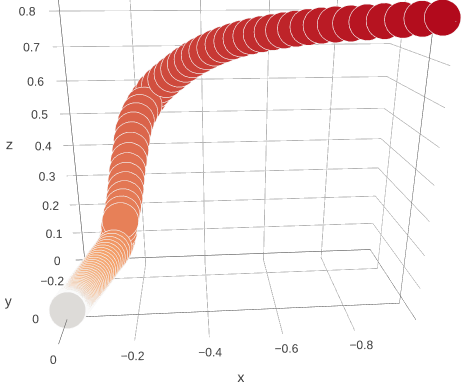
\includegraphics[height=17em]{figures/pickup.png}
\captionof{figure}{Simple visualization of a pickup signal}
}

%----------------------------------------------------------------------------------------

\end{poster}

\end{document}
